% Font options: 10pm, 11pt, 12pt
% Align headings left instead of center: nocenter
\documentclass[xcolor=x11names,compress]{beamer}\usepackage[]{graphicx}\usepackage[]{color}
%% maxwidth is the original width if it is less than linewidth
%% otherwise use linewidth (to make sure the graphics do not exceed the margin)
\makeatletter
\def\maxwidth{ %
  \ifdim\Gin@nat@width>\linewidth
    \linewidth
  \else
    \Gin@nat@width
  \fi
}
\makeatother

\definecolor{fgcolor}{rgb}{0.345, 0.345, 0.345}
\newcommand{\hlnum}[1]{\textcolor[rgb]{0.686,0.059,0.569}{#1}}%
\newcommand{\hlstr}[1]{\textcolor[rgb]{0.192,0.494,0.8}{#1}}%
\newcommand{\hlcom}[1]{\textcolor[rgb]{0.678,0.584,0.686}{\textit{#1}}}%
\newcommand{\hlopt}[1]{\textcolor[rgb]{0,0,0}{#1}}%
\newcommand{\hlstd}[1]{\textcolor[rgb]{0.345,0.345,0.345}{#1}}%
\newcommand{\hlkwa}[1]{\textcolor[rgb]{0.161,0.373,0.58}{\textbf{#1}}}%
\newcommand{\hlkwb}[1]{\textcolor[rgb]{0.69,0.353,0.396}{#1}}%
\newcommand{\hlkwc}[1]{\textcolor[rgb]{0.333,0.667,0.333}{#1}}%
\newcommand{\hlkwd}[1]{\textcolor[rgb]{0.737,0.353,0.396}{\textbf{#1}}}%
\let\hlipl\hlkwb

\usepackage{framed}
\makeatletter
\newenvironment{kframe}{%
 \def\at@end@of@kframe{}%
 \ifinner\ifhmode%
  \def\at@end@of@kframe{\end{minipage}}%
  \begin{minipage}{\columnwidth}%
 \fi\fi%
 \def\FrameCommand##1{\hskip\@totalleftmargin \hskip-\fboxsep
 \colorbox{shadecolor}{##1}\hskip-\fboxsep
     % There is no \\@totalrightmargin, so:
     \hskip-\linewidth \hskip-\@totalleftmargin \hskip\columnwidth}%
 \MakeFramed {\advance\hsize-\width
   \@totalleftmargin\z@ \linewidth\hsize
   \@setminipage}}%
 {\par\unskip\endMakeFramed%
 \at@end@of@kframe}
\makeatother

\definecolor{shadecolor}{rgb}{.97, .97, .97}
\definecolor{messagecolor}{rgb}{0, 0, 0}
\definecolor{warningcolor}{rgb}{1, 0, 1}
\definecolor{errorcolor}{rgb}{1, 0, 0}
\newenvironment{knitrout}{}{} % an empty environment to be redefined in TeX

\usepackage{alltt}
%\documentclass[xcolor=x11names,compress,handout]{beamer}
\usepackage[]{graphicx}
\usepackage[]{color}
\usepackage{booktabs}
\usepackage{hyperref}
\usepackage{tikz}
\usepackage{multirow}
\usepackage{multicol}
\usepackage{dcolumn}
\usepackage{bigstrut}
\usepackage{amsmath} 
\usepackage{xcolor,colortbl}
\usepackage{amssymb}
%\newcommand{\done}{\cellcolor{teal}#1}

%% Beamer Layout %%%%%%%%%%%%%%%%%%%%%%%%%%%%%%%%%%
\useoutertheme[subsection=false,shadow]{miniframes}
\useinnertheme{default}
\usefonttheme{serif}
\usepackage{Arev}
\usepackage{pdfpages}

\setbeamerfont{title like}{shape=\scshape}
\setbeamerfont{frametitle}{shape=\scshape, size=\normalsize}

\definecolor{dkblue}{RGB}{0,0,102}

\setbeamercolor*{lower separation line head}{bg=dkblue} 
\setbeamercolor*{normal text}{fg=black,bg=white} 
\setbeamercolor*{alerted text}{fg=red} 
\setbeamercolor*{example text}{fg=black} 
\setbeamercolor*{structure}{fg=black} 
 
\setbeamercolor*{palette tertiary}{fg=black,bg=black!10} 
\setbeamercolor*{palette quaternary}{fg=black,bg=black!10} 

\renewcommand{\(}{\begin{columns}}
\renewcommand{\)}{\end{columns}}
\newcommand{\<}[1]{\begin{column}{#1}}
\renewcommand{\>}{\end{column}}

\setbeamertemplate{navigation symbols}{} 
\setbeamertemplate{footline}[frame number]
\setbeamertemplate{caption}{\raggedright\insertcaption\par}

\setbeamersize{text margin left=5pt,text margin right=5pt}

\AtBeginSection{\frame{\sectionpage}}
\usepackage{xcolor}
\hypersetup{
    colorlinks,
    linkcolor={red!50!black},
    citecolor={blue!50!black},
    urlcolor={blue!80!black}
}

\setbeamercolor{block title}{use=structure,fg=white,bg=structure.fg!75!orange}
\setbeamercolor{block body}{parent=normal text,use=block title,bg=block title.bg!10!bg}

%%%%%%%%%%%%%%%%%%%%%%%%%%%%%%%%%%%%%%%%%%%%%%%%%%





\title{FLS 6441 - Methods III: Explanation and Causation}
\subtitle{Week 4 - Survey and Lab Experiments}
\author{Jonathan Phillips}
\date{April 2019}
\IfFileExists{upquote.sty}{\usepackage{upquote}}{}
\begin{document}

\frame{\titlepage}

\begin{frame}
\frametitle{Survey and Lab Experiments}
\begin{itemize}
\item Why survey and lab experiments?
\pause
\begin{enumerate}
\item Treatments we cannot administer in reality
\pause
\item Random treatment assignment not permitted in reality
\pause
\item Outcome measurements that are hard to take in reality
\pause
\item Reduce variation in context and noise in data
\pause
\item To generalize beyond specific situations to abstract behaviour
\end{enumerate}
\end{itemize}
\end{frame}

\section{Lab Experiments}

\begin{frame}
\frametitle{Lab Experiments}
\begin{itemize}
\item \textbf{Treatment Assignment}: Same as a Field Experiment
\pause
\item \textbf{Treatment}: Not a manipulation of real world political or economic processes, but establishing controlled 'lab' conditions
\pause
\begin{itemize}
\item The advantage: Control over context helps isolate mechanisms
\pause
\item The disadvantage: Can we generalize to the real world?
\end{itemize}
\end{itemize}
\end{frame}

\begin{frame}
\frametitle{Lab Experiments}
\begin{itemize}
\item Problems generalizing from the lab:
\pause
\begin{itemize}
\item \textbf{Hawthorne effect}: Lab context influences behaviour, social desirability bias
\pause
\item \textbf{Context effects}: The real-world always provides more information, more history
\pause
\item \textbf{Process effects}: People care \textit{how} decisions are made
\item \textbf{Selection effects}: Actors in specific roles are rarely representative samples, 'WEIRD' or pro-social lab subjects
\end{itemize}
\end{itemize}
\end{frame}

\begin{frame}
\frametitle{Lab Experiments}
\begin{itemize}
\item The lab differs from the field 
\pause
\begin{itemize}
\item The stakes
\pause
\item The norms (specific norms of being an experimental subject)
\pause
\item The degree of scrutiny
\pause
\item The sample of individuals
\pause
\item The degree of anonymity
\end{itemize}
\end{itemize}
\end{frame}

\begin{frame}
\frametitle{Lab Experiments}
\begin{itemize}
\item Lab experiments are \textit{inherently} imperfect (Levitt and List 2006)
\pause
\item Decisions change depending on the degree of \textbf{scrutiny}
\pause
\begin{itemize}
\item ``You tip more when you're on a date''
\pause
\item Social norms are activated, eg. treating one-shot games like repeated games
\pause
\item Scrutiny alters who wants to make a decision as well as the decision they make
\pause
\item Subjets use cues (heuristics) to draw on 'similar' situations from the real world
\end{itemize}
\end{itemize}
\end{frame}

\begin{frame}
\frametitle{Lab Experiments}
\begin{itemize}
\item Many studies find more cooperation in the lab than in the real world
\pause
\begin{itemize}
\item Scrutiny increases cooperation
\pause
\item Anonymity reduces cooperation
\pause
\item That's interesting in itself! We can manipulate the degree of scrutiny/anonymity etc.
\end{itemize}
\pause
\item Lab experiments may be generalizable where norms/morality is less important (???)
\end{itemize}
\end{frame}

\begin{frame}
\frametitle{Lab-in-the-Field Experiments}
\begin{itemize}
\item In a natural setting with the target population
\pause
\item Standardized, artificial treatment and measurement
\end{itemize}
\end{frame}

\begin{frame}
\frametitle{Lab-in-the-Field Experiments}
\begin{itemize}
\item Habyarimana et al (2007)
\pause
\item Existing consensus: Ethnic diversity -> \textbf{Less} public goods provision
\pause
\item But how? Theories:
\pause
\begin{itemize}
\item Preferences - in-group fairness
\item Technology - social networks permit identification and sanctioning
\item Strategy Selection - choose to cooperate more often
\end{itemize}
\end{itemize}
\end{frame}

\begin{frame}
\frametitle{Lab-in-the-Field Experiments}
\begin{itemize}
\item Lab-in-the-field
\item \textbf{Population}: Ugandans
\item \textbf{Sample}: 300 people in a diverse area with few public goods
\item \textbf{Treatment/Control}: Various Games
\item \textbf{Treatment assignment}: Random assignment to co-ethnic/non-co-ethnic
\end{itemize}
\end{frame}

\begin{frame}
\frametitle{Lab-in-the-Field Experiments}
\begin{itemize}
\item \textbf{Preferences} - dictator game between self and two others
\begin{itemize}
\item No bias towards co-ethnics
\pause
\end{itemize}
\item \textbf{Technology 1, productivity} - teamwork in a puzzle requiring communication
\begin{itemize}
\item Co-ethnic teams don't perform any better
\pause
\end{itemize}
\item \textbf{Technology 2, social networks} - Can you find a co-ethnic in the town faster than a non-co-ethnic?
\begin{itemize}
\item  Yes (43\% vs 28\% success)
\pause
\end{itemize}
\item \textbf{Strategy Selection} - Does anonymity for the sender in the dictator game make a difference?
\begin{itemize}
\item Yes - offer more to co-ethnics when offerers believe they can be seen
\pause
\end{itemize}
\end{itemize}
\end{frame}

\begin{frame}
\frametitle{Lab-in-the-Field Experiments}
\begin{itemize}
\item \textbf{Conclusion:} Norms and Networks allow co-ethnics to provide more public goods
\pause
\begin{itemize}
\item ...But where are the public goods here?
\item Are public goods organized by voluntary contributions or coercive central authority?
\item Is this true of all parts of Kampala? Uganda? All ethnic groups?
\end{itemize}
\end{itemize}
\end{frame}

\section{Survey Experiments}

\begin{frame}
\frametitle{Survey Experiments}
\begin{itemize}
\item Treatment occurs \textit{within} the survey questionnaire
\pause
\item Outcome measurement also \textit{within} the survey questionnaire
\pause
\begin{itemize}
\item Different versions of the questionnaire randomly applied
\pause
\item Not a field experiment: Still an artificial context
\pause
\item Not a lab experiment: People not brought to a single location or interacting
\end{itemize}
\end{itemize}
\end{frame}

\begin{frame}
\frametitle{Survey Experiments}
\begin{itemize}
\item Easy and cheap to implement
\pause
\item Can be targeted to our real population of interest
\pause
\item But a limited range of 'weak' treatments possible
\pause
\item And we can only measure short-term effects
\end{itemize}
\end{frame}

\begin{frame}
\frametitle{Survey Experiments}
\begin{itemize}
\item Humans are subject to psychological and social influences
\pause
\item These create threats to estimating causal effects
\pause
\begin{itemize}
\item \textbf{Social Desirability Bias:} Respondents lie when they think someone is listening to their answers! (Including the enumerator)
\pause
\item \textbf{Sequencing Bias:} If we ask about who you voted for after twenty questions about redistribution and equality, your answer might be different
\pause
\item \textbf{Acquiescence Bias:} Thinking about your answers is hard, so it's easier just to agree with the default/first option
\pause
\item \textbf{Anchoring Bias:} The first piece of information in a question affects our response, Eg. The average person does x, what do you do?
\end{itemize}
\end{itemize}
\end{frame}

\begin{frame}
\frametitle{Types of Survey Experiments}
\begin{itemize}
\item But we can also use these influences to our advantage to study psychological and social processes:
\pause
\end{itemize}
\begin{enumerate}
\item \textbf{Framing Experiments} - how responses vary to question content
\pause
\item \textbf{Priming Experiments} - to measure the effect of a prime on a response to a fixed question
\pause
\item \textbf{List Experiments} - to reduce social desirability bias in measurement
\pause
\item \textbf{Conjoint Experiments} - to measure relative preferences
\end{enumerate}
\end{frame}

\begin{frame}
\frametitle{1. Framing}
\begin{itemize}
\item How much do details in the question affect our responses?
\pause
\item (i) Town A has only \textbf{80\%} of the income of Town B, and the gap is widening. The government proposes to transfer income from Town A to Town B to reduce inequality. How much do you think would be a fair tax on Town A's income?
\pause
\item (ii) Town A has only \textbf{20\%} of the income of Town B, and the gap is widening. The government proposes to transfer income from Town A to Town B to reduce inequality. How much do you think would be a fair tax on Town A's income?
\pause
\item 1\%
\item 5\%
\item 10\%
\item 25\%
\item 50\%
\end{itemize}
\end{frame}

\begin{frame}
\frametitle{1. Framing}
\begin{itemize}
\item Within/Between Survey Experiments
\pause
\item Between: Treated and Control are different people
\pause
\item Within: Treated and Control measures from the same person
\begin{itemize}
\item But aren't these different 'units'?? \pause Yes!
\pause
\item But the time difference is usually just a few minutes, so maybe more plausible
\pause
\item More problematic is sequencing bias
\pause
\item But we can also randomize the sequence
\end{itemize}
\end{itemize}
\end{frame}

\begin{frame}
\frametitle{2. Priming}
\begin{itemize}
\item The entire point of survey bias is that the questions we ask change the answers we get
\pause
\item So changing questions across respondents might change \textit{ALL} subsequent responses
\pause
\item We design a prior task that creates an \textit{unconscious} bias in subsequent answers
\pause
\item The treatment/control prime is separated from the response question
\pause
\begin{itemize}
\item Usually the prime is a few questions before the response
\pause
\item Everyone sees the same response question
\end{itemize}
\end{itemize}
\end{frame}

\begin{frame}
\frametitle{2. Priming}
\begin{itemize}
\item Eg. If we want to measure the effect of 'hope' vs. 'fear' on the demand for constitutional reform:
\pause
\item There are good reasons to be hopeful for democracy: More people voted than ever before in the 2018 election, suggesting strong citizen participation in democracy. Did you vote in 2018?
\pause
\item Many people fear for the survival of democracy: The proportion of voters who turned out to vote fell again in the 2018 election, suggesting a critical problem of declining trust and engagement in democracy. Did you vote in 2018?
\pause
\item How much do you support constitutional reform?
\end{itemize}
\end{frame}

\begin{frame}
\frametitle{3. List Experiments}
\begin{itemize}
\item Most survey responses are biased to give the answer they think the researcher wants
\pause
\begin{itemize}
\item \textbf{Social desirability bias} has \textit{differential} effects across respondents and topics
\begin{itemize}
\item Most people say they recycle, even though they do not
\pause
\item But rich people exaggerate more than poor people
\end{itemize}
\pause
\end{itemize}
\item List experiments make individual responses \textit{invisible} to the researcher
\pause
\begin{itemize}
\item Knowing this, hopefully the respondent answers more accurately
\end{itemize}
\end{itemize}
\end{frame}

\begin{frame}
\frametitle{3. List Experiments}
I am now going to read out a list of activities. Please count the number of these activities that you have done in the past one year. Please do not tell me WHICH activities you have done, only the TOTAL NUMBER of them: 
\begin{itemize}
\item Voted
\item Attended a Town Hall Meeting
\item Travelled to the State Capital
\end{itemize}
\end{frame}

\begin{frame}
\frametitle{3. List Experiments}
 I am now going to read out a list of activities. Please count the number of these activities that you have done in the past one year. Please do not tell me WHICH activities you have done, only the TOTAL NUMBER of them:
\begin{itemize}
\item Voted
\item Attended a Town Hall Meeting
\item Been offered a gift, some food or money in exchange for your vote; 
\item Travelled to the State Capital
\end{itemize}
\end{frame}

\begin{frame}
\frametitle{3. List Experiments}
\begin{itemize}
\item \item Eg. Gonzalez-Ocantos (2010) - list experiment on vote-buying in Nicaragua 2008 municipal elections
\item \textbf{Direct Question}: Have you received a gift or favour in exchange for your vote?
\begin{itemize}
\item 3\%
\pause
\end{itemize}
\item \textbf{List experiment}:
\begin{itemize}
\item Just the difference in mean responses between treatment and control lists
\item 24\% = 2.31 - 2.06
\end{itemize}
\end{itemize}
\end{frame}

\begin{frame}
\frametitle{3. List Experiments}
\textbf{Assumptions:}
\begin{enumerate}
\item No Liars - People answer honestly in the presence of the sensitive item
\pause
\begin{itemize}
\item Do respondents really understand anonymity?
\end{itemize}
\pause
\item No Ceiling effects - '4' means my answers are no longer anonymous; instead report '3'
\pause
\item No Floor Effects - If the control items are rare, respondents may be reluctant to report '1' and choose '0' instead.
\pause
\item No Design Effects- Presence of the treatment item doesn't affect answers on other items
\begin{itemize}
\item Bias towards a 'reasonable'/central number?
\end{itemize}
\end{enumerate}
\end{frame}

\begin{frame}
\frametitle{4. Conjoint Survey Experiments}
\begin{itemize}
\item How do people make choices between many options?
\pause
\item Treatments are often 'bundles' of characteristics, but which aspect matters most?
\pause
\item Also a problem of social desirability bias in which characteristics matter
\end{itemize}
\end{frame}

\begin{frame}
\frametitle{4. Conjoint Survey Experiments}
\begin{itemize}
\item Hainmueller et al 2013 - How do attitudes to immigrants depend on immigrant characteristics?
\pause
\item Vary education, profession, language, gender, national origin, etc.
\pause
\item Profiles
\begin{itemize}
\item Attributes
\begin{itemize}
\item Values
\end{itemize}
\end{itemize}
\pause
\item Randomize values and attribute order to prevent bias
\pause
\item Treatment is the \textbf{combination} of attributes the respondent sees
\pause
\item Millions of possible treatments
\end{itemize}
\end{frame}

\setbeamercolor{background canvas}{bg=}
\includepdf[pages={6}]{Jens.pdf}

\setbeamercolor{background canvas}{bg=}
\includepdf[pages={21}]{Jens.pdf}

\begin{frame}
\frametitle{4. Conjoint Survey Experiments}
\begin{itemize}
\item Estimating results uses a simple regression of respondent choices on profile attribute-values
\pause
\item But each specific profile (treatment) may arise too rarely to make comparisons of individual attribute-values
\pause
\begin{itemize}
\item So this is \textbf{not} an Average Treatment Effect for each profile
\pause
\item Eg. the effect of gender when age, language etc. are held constant
\pause
\item It is an \textbf{Average Marginal Component Effect}
\pause
\item Eg. the effect of gender averaging across all possibilities of age, language, etc.
\end{itemize}
\end{itemize}
\end{frame}

\begin{frame}
\frametitle{4. Conjoint Survey Experiments}
Assumptions:
\begin{itemize}
\item We're still assuming people try to answer honestly
\pause
\item The ordering of attributes does not matter (or is randomized)
\pause
\item Profiles are randomized
\end{itemize}
\end{frame}

\section{Generalizability}

\begin{frame}
\frametitle{Generalizability}
\begin{itemize}
\item Can we generalize from survey/lab responses to real-world behaviour?
\pause
\item \textbf{Non-Behavioural Measures:} 
\begin{itemize}
\item What is at stake in the answer? Are there any actual consequences? 
\pause
\item Will they have to defend their answer in the community later?
\pause
\item Cognitive costs of thinking about your response
\pause
\item 'Cheap talk'
\end{itemize}
\end{itemize}
\end{frame}

\begin{frame}
\frametitle{Generalizability}
\begin{itemize}
\item Can we generalize from survey/lab responses to real-world behaviour?
\pause
\item \textbf{Credibility:} 
\begin{itemize}
\pause
\item 'Treatments' in survey experiments are just information or wording
\pause
\item But do respondents 'believe' that information?
\pause
\item Do they have conflicting information? What is their 'prior'?
\pause
\item What 'authority' or 'trust' does the source (you!) have?
\end{itemize}
\end{enumerate}
\end{itemize}
\end{frame}

\begin{frame}
\frametitle{Generalizability}
\begin{itemize}
\item Can we generalize from survey/lab responses to real-world behaviour?
\pause
\item \textbf{Context:} 
\begin{itemize}
\pause
\item Our interpretation of treatments depends on subtle signals - someone telling you a Trump voter is moving in next door is very different to actually meeting that person
\pause
\item We want to abstract from that complexity, but are humans capable of reporting their 'average' responses?
\end{itemize}
\end{enumerate}
\end{itemize}
\end{frame}

\begin{frame}
\frametitle{Generalizability}
\begin{itemize}
\item Can we generalize from survey/lab responses to real-world behaviour?
\pause
\item \textbf{Durability:} 
\begin{itemize}
\pause
\item We find that a nationalism prompt produces pro-statist attitudes five minutes later in a survey
\pause
\item Would that effect persist one hour later?
\pause
\item How about a year later?
\pause
\item Real-world treatments are often continuous or repeated
\end{itemize}
\end{enumerate}
\end{itemize}
\end{frame}

\begin{frame}
\frametitle{Generalizability}
\begin{itemize}
\item How reliable are the responses to a Conjoint Experiment?
\pause
\begin{itemize}
\item Stated preferences vs. Revealed preferences
\end{itemize}
\pause
\item Hainmueller et al 2014 - compare conjoint responses to a Swiss referendum
\pause
\item Citizens voted on specific naturalization applicants (Really!)
\end{itemize}
\end{frame}

\setbeamercolor{background canvas}{bg=}
\includepdf[pages={22}, scale=1.6, offset=0 -2.5cm]{Hainmueller2014.pdf}

\begin{frame}
\frametitle{Generalizability}
\begin{itemize}
\item But note the conjoint method still hugely under-estimated the overall rejection rate
\item 21\% versus 37\% in reality
\end{itemize}
\end{frame}

\end{document}


% Anchoring vignettes - where place self on idelogical scale? Conservatives and Liberals interpret the scale differently so can't compare. So ask where to put hypothetical or real people so can calibrate.
% Problems of online survey experiments: 'nationally representative'?
% How long do effects last?
% We might interpret treatment wrongly, eg. we put a black name and actually respondents interpret as a rich name
% Satisficing - costs to think through questions and no reward, so satisfice
% Mention incentives

%setwd('C:\\Users\\Jonny\\Google Drive\\Academic\\USP\\Class\\Week 1 - Intro\\Lecture Slides')
%knitr::knit("Slides_Wk1_intro_5.Rnw")
